\documentclass[12pt,a4paper]{book}

               %%%%%%%%%%%%%%%%%%%%%%%%%%%%%%%%%%%%%%
               %    Scelta dei package da usare     %
               %%%%%%%%%%%%%%%%%%%%%%%%%%%%%%%%%%%%%%

\usepackage[italian]{babel}
\usepackage[latin1]{inputenc}
\usepackage{amsmath,amsfonts,amssymb,amsthm}
\usepackage{deistesi}
\usepackage{fancyhdr}
\usepackage{hyperref}
\usepackage{cleveref}
\usepackage{listings}
\usepackage{caption}
\captionsetup[lstlisting]{font={small,tt}}
               %%%%%%%%%%%%%%%%%%%%%%%%%%%%%%%%%%%%%%%%
               % Scelta delle dimensioni della pagina %
               %%%%%%%%%%%%%%%%%%%%%%%%%%%%%%%%%%%%%%%%

\setlength{\textwidth}{13.5cm}
\setlength{\textheight}{19cm}
\setlength{\footskip}{3cm}




               %%%%%%%%%%%%%%%%%%%%%%%%%%%%%%%%%%%%%%
               %  Informazioni generali sulla Tesi  %
               %    da usare nell'intestazione      %
               %%%%%%%%%%%%%%%%%%%%%%%%%%%%%%%%%%%%%%

\titolo{FoodOn}
\laureando{Lorenzo Chiana}
\annoaccademico{2019--2020}
\facolta{CAMPUS DI CESENA\\SCUOLA DI INGEGNERIA}
\corsodilaurea{Ingegneria e Scienze Informatiche}
\corso{Web Semantico}
%\relatore{Alessandro Ricci}


\begin{document}

%%%%%%%%%%%%%%%%%%%%%%%%%
% inizio prefazione
%
% pagina del titolo, indice, sommario
%%%%%%%%%%%%%%%%%%%%%%%%%
\frontmatter
\maketitle
\pagestyle{plain} 
\tableofcontents
%``testo''


%%%%%%%%%%%%%%%%%%%%%%%%%
% inizio corpo del documento
%
% sequenze dei vari capitoli
% � consigliato mantenere una struttura logica ben definita per separare i vari capitoli
% si consiglia di reificare tale struttura fisicamente sul file system
%%%%%%%%%%%%%%%%%%%%%%%%%

\mainmatter

% stile della pagina
\pagestyle{fancy} \fancyhead[LE,RO]{\bfseries\thepage}

\chapter{Introduzione}

\section{Cause}

\index{Cause}

Al giorno d'oggi la costruzione di reti progettate per la condivisione ad alta capacit� di dati e il fatto che la comunicazione e la diffusione di concetti viene maggiormente veicolata attraverso l'uso di computer e di tecnologie simili, hanno permesso lo scambio sempre pi� crescente di dati governativi e commerciali mettendo, per�, in luce un problema fondamentale: la molteplicit� di lingue e di dizionari di dati.\\
Questo problema comporta un blocco del contenuto delle informazioni esistenti e connesse ad Internet e la mancanza di una lingua franca digitale � evidente nel dominio del cibo, poich� i materiali viaggiano dalla loro provenienza, agricola o meno, ai consumatori attraverso catene di processo e di distribuzione.\\
Un vocabolario bene definito e gerarchico, con relazioni logiche, ossia un'ontologia, � necessario per aiutare ad armonizzare quei dati che abbracciano i settori della sicurezza, qualit�, produzione e distribuzione alimentare e, di conseguenza, della salute e convenienza dei consumatori.

\section{FoodOn}

\index{FoodOn}

% inclusione dei capitoli
\chapter{FoodOn}

\section{Ontologia}
\index{Ontologia}
\section{Struttura}
\index{Struttura}
\section{Funzionalit�}
\index{Funzionalit�}


\chapter{Tecnologie}
In questo capitolo si vanno ad affrontare tutte le tecnologie utilizzate in questo progetto quali: RDF, RDFS, OWL, OWLAPI, SWRL, HermiT OWL Reasoner; dando anche una loro spiegazione.
\section{RDF}
\index{RDF}
Resource Description Framework o, abbreviato, RDF \`e lo strumento base proposto da W3C per la codifica, lo scambio e il riutilizzo di metadati strutturati che permette di descrivere le relazioni fra le entit\`a della parte di realt\`a che si vuole modellare.
In questa tecnologia l'unit\`a base per rappresentare l'informazione \`e lo \textit{statement}, ossia una tripla del tipo \textit{Soggetto - Predicato - Oggetto}.
In questa tripla il soggetto e l'oggetto rappresentano una risorsa e il predicato la relazione tra esse. \cite{rdf}

\begin{figure}[h!]
    \centering
    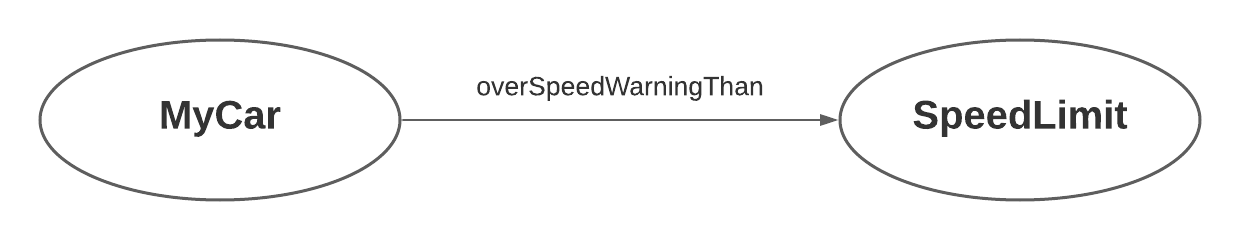
\includegraphics[width=0.90\textwidth]{img/overSpeedWarningThanRDF.png}
   	\caption{Tripla RDF con soggetto \textit{MyCar}, predicato \textit{overSpeedWarningThan} e oggetto \textit{SpeedLimit}}.
	\label{fig:triplaRDF}
\end{figure}

\section{RDFS}
\index{RDFS}
RDFS, acronimo di RDF Schema, \`e una tecnologia nata dall'esigenza di dover definire vocabolari e semantiche, cosa che non \`e possibile fare solo con RDF.
RDF Schema definisce un insieme di risorse RDF da usare per descrivere caratteristiche di altre risorse e propriet\`a RDF. \cite{rdfs}

\section{OWL}
\index{OWL}
OWL, acronimo di Web Ontology Language, \`e nato dall'esigenza di avere maggior potere espressivo rispetto a RDFS.
I componenti principali di un'ontologia OWL sono tre: individui, propriet\`a e classi. Gli individui rappresentano gli oggetti nel dominio di interesse, le propriet\`a sono relazioni binarie (ovvero che collegano due oggetti per volta) tra individui, le classi sono gruppi di individui.
\cite{owl}

\section{OWLAPI}
\index{OWLAPI}
OWLAPI \`e un'API per Java 8 nata per la creazione, la manipolazione e la serializzazione di ontologie OWL.
L'ultima versione si focalizza su OWL 2.
Vi \`e una ampia documentazione con tanto di esempi pratici nel loro repository (\url{https://github.com/owlcs/owlapi/wiki/Documentation}).

\section{SWRL}
\index{SWRL}
SWRL, acronico di Semantic Web Rule Language, \`e un linguaggio che consente la creazione di regole espresse in termini di concetti OWL (classi, propriet\`a, individuals).
Ci\`o fornisce una capacit\`a di ragionamento deduttivo pi\`u potente al solo utilizzo di OWL. 
SWRL supporta solo l'inferenza monotonica:
\begin{itemize}
\item le regole non possono essere utilizzate per modificare le informazioni esistenti in un'ontologia;
\item le regole non possono ritirare o rimuovere informazioni da un'ontologia.
\end{itemize}
Una regola SWRL \`e composta da una parte antecedente (il corpo) e da una parte conseguente (la testa), entrambi costituiti da congiunzioni positive di atomi.
Un atomo \`e espresso nella seguente forma: p(arg1, arg2, ..., argN) dove p \`e il simbolo del predicato e tra parentesi vi sono gli argomenti dell'espressione.\cite{swrl}

Esempi applicati al progetto:\\
\textbf{Mantenere una velocit\`a costante}\\
\begin{center}
\emph{isRunningOn(?X, ?Lane) $\char`\^$ OneWayLane(?Lane) $\char`\^$ SpeedLimit(?Y) $\char`\^$ overSpeedWarningThan(?X, ?Y) $\rightarrow$ constantSpeed(?X)}\\
\end{center}
In questo caso il body \`e rappresentato da tutto ci\`o che \`e antecedente alla freccia e la head da ci\`o che ne viene dopo.
Con questa regola il reasoner inferir\`a che se la head risulta vera allora anche il body lo sar\`a.
Nello specifico se esiste una tripla che:
\begin{enumerate}
\item associa le variabili \textit{X} e \textit{Lane} con la propriet\`a \textit{isRunningOn};
\item \textit{Lane} \`e istanza della classe \textit{OneWayLane};
\item \textit{Y} \`e istanza della classe \textit{SpeedLimit};
\item associa \textit{X} e \textit{Y} alla propriet\`a \textit{overSpeedWarningThan};
\end{enumerate}
allora \textit{X} deve mantenere una velocit\`a costante.\\
\textbf{Accelerare}\\
\begin{center}
\emph{isRunningOn(?X, ?Lane) $\char`\^$ OneWayLane(?Lane) $\rightarrow$ acceleration(?X)}\\
\end{center}
In questo caso la tripla che deve esistere per far s\`i che \textit{X} acceleri deve associare le variabili \textit{X} e \textit{Lane} con la propriet\`a \textit{isRunningOn} e che \textit{Lane} sia istanza di \textit{OneWayLane}.

\section{HermiT OWL Reasoner}
\index{HermiT}
HermiT \`e un reasoner per ontologie scritto in OWL.
Data una ontologia OWL HermiT \`e in grado di determinare se essa sia coerente o meno, identificare le relazioni di inclusione tra le classi e molto altro.
HermiT \`e il primo reasoner OWL disponibile pubblicamente basato sul nuovo calcolo ``hypertableau'' che fornisce un ragionamento molto pi\`u efficiente di qualsiasi algoritmo precedentemente noto. \cite{hermit}
Per i motivi sopracitati e per la grande disponibilit\`a di esempi trovati online anche, e soprattutto, dei vari esempi nella documentazione all'interno del Wiki del repository ufficiale di OWLAPI, la scelta del reasoner \`e ricaduta su HermiT.

%\appendix

% inclusione dei capitoli
%\chapter{FoodOn}

\section{Ontologia}
\index{Ontologia}
\section{Struttura}
\index{Struttura}
\section{Funzionalit�}
\index{Funzionalit�}



%%%%%%%%%%%%%%%%%%%%%%%%%
% inizio parte finale del documento
%
% eventuali appendici, bibliografia obbligatoria,
% eventuale lista delle tabelle e delle figure (nel caso decommentare la riga con i comandi \listoffigures e \listoftables)
%%%%%%%%%%%%%%%%%%%%%%%%%
\backmatter


%\input{./Appendice/appendice.tex}
% \input{./Bibliografia/bibliografia.tex}


%\listoffigures
%\listoftables

% chiusura del documento
\end{document}
